% \vspace*{1mm}
\section{Introduction}
% \vspace*{1mm}
%%% Motivation on machine unlearning vs. data privacy and influence of data points

Machine unlearning (\textbf{\MU}) initiates a reverse learning process to scrub the influence of   data points   from a trained machine learning (\textbf{ML}) model. It was  introduced to avoid information leakage about private   data upon completion of training \cite{cao2015towards, bourtoule2021machine, nguyen2022survey},
%particularly 
%The need of {\MU}  grows    
%in coming forth with 
particularly in compliance with
legislation like `the right to be forgotten' \cite{rosen2011right} in General Data Protection Regulation (GDPR) \cite{hoofnagle2019european}.
%\PS{I didn't follow the phrase ``in coming forth with'' in the previous sentence. How about: ``... particularly in compliance with legislation ...''}
%, and    California Consumer Privacy Act (CCPA) \cite{pardau2018california}. 
The  \textit{direct but optimal} unlearning approach  is \textit{exact unlearning} to \textit{retrain}   ML models from scratch using the  remaining training set, after removing the data points to be scrubbed.
%\PR{``naive but optimal'' $\to$ ``direct but optimal''? ``naive'' might have a negative connotation} 
Although retraining yields the \textit{ground-truth} unlearning strategy, it is the most computationally intensive one.
%\SL{Another possible limitation of retraining is that the trainer needs complete access to the full retrained dataset.}
%\PR{Another disadvantage of retraining is that trainer needs complete access to original training data. Ideally, trainer should only need the forget set, and maybe a bit of retained set.}
Therefore,   the development of \textit{approximate but fast} unlearning methods   has  become a  major focus in research \cite{warnecke2021machine,graves2021amnesiac,thudi2021unrolling,becker2022evaluating,izzo2021approximate}.






%%% Existing methods and key challenges remaining
%% challenges in approximate unlearning
Despite the computational benefits of  approximate unlearning, it often  lacks a strong guarantee on the effectiveness  of unlearning, resulting in a performance gap with  exact unlearning \cite{thudi2022necessity}.  In particular, we encounter two main challenges.
%\PR{``suffer'' $\to$ ``face'' or ``encounter''}
\textit{First}, the performance of approximate unlearning   can heavily rely on the configuration of algorithmic parameters.
%\PR{``could heavily rely'' $\to$ ``can heavily rely'' or ``heavily relies''}
For example, the Fisher forgetting method \cite{golatkar2020eternal} needs to carefully tune the Fisher information regularization parameter  in each   data-model setup.  
\textit{Second}, the effectiveness of an approximate scheme can vary significantly across the different unlearning evaluation criteria, and their trade-offs are not well understood. For example,  high `efficacy' (ability to protect the privacy of the scrubbed data)
%\PS{this description in parenthesis should come when efficacy is mentioned for the first time at the beginning of this para.} 
\textit{neither} implies \textit{nor} precludes high `fidelity' (accuracy on the remaining dataset) \cite{becker2022evaluating}. This raises our \textbf{driving question (Q)}  below:
% \textit{Second}, the effectiveness of approximate unlearning also varies  using different unlearning criteria \cite{becker2022evaluating}, \textit{e.g.}, evaluation by forgetting data information contained in the unlearned model (termed `efficacy' by \citet{becker2022evaluating}) versus  accuracy on the remained dataset (termed `fidelity' by \citet{becker2022evaluating}).
% \PR{How about ``Second, the effectiveness of an approximate scheme can vary significantly across the multiple unlearning evaluation criteria and their tradeoffs are not well understood -- for example,  high `efficacy' (ability to protect the privacy of the scrubbed data) \underline{does not imply {\bf or} preclude} high `fidelity' (accuracy on remaining data).''}
%Spurred by the above,  we ask:
%\PR{How about ``This brings us to our driving question.''}
% \vspace*{2mm}
\vspace*{3mm}
\begin{tcolorbox}[before skip=-2.1mm, after skip=0.2cm, boxsep=0.0cm, middle=0.1cm, top=0.1cm, bottom=0.1cm]
%\vspace*{1mm}
\textbf{(Q)} \textit{Is there a theoretically-grounded and broadly-applicable method to improve approximate unlearning across different unlearning criteria?}
%\vspace*{1mm}
\end{tcolorbox}
%\PS{Minor point: aren't ``general'' and ``broadly applicable'' redundant?}



%to the best of our knowledge, there does not exist any theoretically-grounded and  broadly-applicable approaches to improve approximate unlearning across multi-faceted unlearning metrics. By contrast, 

To address \textbf{(Q)}, we advance {\MU} through a fresh and novel viewpoint: \textbf{model sparsification}. \textit{Our key finding} is that model sparsity (achieved by weight pruning) can significantly reduce the gap between approximate unlearning and exact unlearning; see \textbf{Fig.\,\ref{fig: results_highlights}} for the schematic overview of our proposal
and  highlighted empirical performance.

\begin{wrapfigure}{r}{80mm}
\vspace*{-4mm}
\centerline{
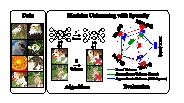
\includegraphics[width=80mm,height=!]{figs/overview_new.pdf}
}
% \hspace*{-2mm}
\vspace*{-2mm}
\caption{\footnotesize{
Schematic overview of our proposal on model sparsity-driven {\MU}. Evaluation at-a-glance shows the performance of three unlearning methods (retraining-based exact unlearning, finetuning-based approximate unlearning \cite{golatkar2020eternal}, 
and proposed   unlearning on 95\%-sparse model) under five metrics:  
unlearning accuracy ({\UA}), membership inference attack (MIA)-based unlearning efficacy, accuracy on remaining data ({\RA}), testing accuracy (\TA), and run-time efficiency (\RTE); see summary in \textbf{Tab.\,\ref{tab: summary_MU_methods_metrics}}.
The unlearning scenario is given by class-wise forgetting, where data points of a single class are scrubbed.  Each metric is normalized to $[0,1]$ based on the best result across unlearning methods 
  for ease of visualization.
  %, while the actual best value  is provided.
%Each performance metric is normalized to $[0,1]$ based on the best result  across unlearning methods.
%We normalized each metric by dividing the best performance in that metric, and $100\%$ denotes the best performance on each metric. 
Results indicate that \textcolor{blue}{model sparsity} reduces the gap between \textcolor{red}{exact} and \textcolor{ForestGreen}{approximate} {\MU} without loss in efficiency. 
%\JC{[updated]}
% \SL{change to 95\%-sparse case.}
% \JC{Add l1-sparse unlearn?} \SL{[Yes. You can use $\ell_1$ to replace `95\% sparse finetuning'.]}
% \SL{talk to me about this figure.}
%\JC{An overview of our method (briefly describe the figure) ... The radar chart on the right gathered the evaluation metrics at a glance. (Describe all metrics, especially MIA)} 
%\SL{[@Yuguang, @Jiancheng, @Jinghan. Talk to me.]} 
%\YL{annotating the five metrics in the captions would be helpful..}
%\PS{How come dense model unlearning is not a pentagon in the radar chart? Or is it hidden behind sparsity aware pentagon?}
}}
\label{fig: results_highlights}
%\end{wrapfigure}
%\end{figure}
\vspace{-7.1mm}
\end{wrapfigure}
%\vspace*{-8mm}
% \begin{figure}[htb]
% %\begin{wrapfigure}{r}{80mm}
% %\vspace*{-6mm}
% \centerline{
% %\begin{tabular}{cc}
% %\hspace*{0mm}\includegraphics[width=.3\textwidth,height=!]{figure/performance_comparison.pdf}  
% %&
% %\hspace*{-4mm}
% 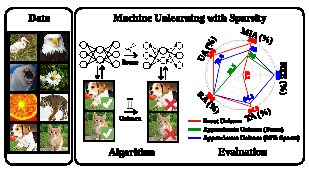
\includegraphics[width=.49\textwidth,height=!]{figs/Overview.pdf}
% % \\
% % \hspace*{2mm}\footnotesize{(a) Test accuracy vs. pruning ratio.} &   \footnotesize{(b) Runtime of pruning.}
% %\end{tabular}
% }
% \vspace*{-3mm}
% \caption{\footnotesize{
% %\JC{"95\% Sparse" -> "Sparse" in the figure}
% Schematic overview of our proposal on model sparsity-driven {\MU}. Performance at-a-glance is provided when evaluating three unlearning methods (retraining-based exact unlearning, finetuning-based approximate unlearning \cite{golatkar2020eternal}, 
% and proposed finetuning-based  unlearning on 95\%-sparse model) under five   metrics,  
% unlearning accuracy ({\UA}), membership inference attack (MIA)-based unlearning efficacy, accuracy on remaining data ({\RA}), testing accuracy (\TA), and run-time efficiency (\RTE), as will be shown in Table\,\ref{tab: summary_MU_methods_metrics}. Results show that \textcolor{blue}{model sparsity} reduces the gap between \textcolor{red}{exact} and \textcolor{ForestGreen}{approximate} {\MU}.
% %\JC{An overview of our method (briefly describe the figure) ... The radar chart on the right gathered the evaluation metrics at a glance. (Describe all metrics, especially MIA)} 
% %\SL{[@Yuguang, @Jiancheng, @Jinghan. Talk to me.]} 
% %\YL{annotating the five metrics in the captions would be helpful..}
% %\PS{How come dense model unlearning is not a pentagon in the radar chart? Or is it hidden behind sparsity aware pentagon?}
% }}
% \label{fig: results_highlights}
% %  \vspace*{-3.8mm}
% %\end{wrapfigure}
% %\end{figure}
% \end{figure}

Model sparsification (or weight pruning) has been extensively studied   in the literature \cite{han2015deep, chen2021lottery, frankle2018lottery, frankle2020linear, ma2021sanity, zhang2022advancing, blalock2020state}, 
focusing on the interrelation between model compression and generalization.
%but with a focus on    model efficiency (\textit{i.e.}, reducing model sizes by removing redundant parameters) versus sparse model's generalization ability.
%\PR{Can we say ``... studied in literature, focusing on the tradeoff between model compression and generalization.''}
For example, the notable lottery ticket hypothesis (\textbf{LTH})  \cite{frankle2018lottery} demonstrated 
the existence of a sparse subnetwork (the so-called `winning ticket') that matches or even exceeds the test accuracy of the original dense model. In addition to generalization, the impact of pruning has also been investigated on model robustness \cite{sehwag2020hydra,chen2022quarantine,diffenderfer2021winning}, fairness \cite{stoychev2022effect,xu2022can}, interpretability \cite{wong2021leveraging,chen2022can}, loss landscape \cite{frankle2020linear,chen2022can}, and privacy \cite{huang2020privacy,wang2020against}. In particular, 
the privacy gains from pruning \cite{huang2020privacy,wang2020against} imply connections between data influence and model sparsification.

% the gain of privacy   from pruning   \cite{huang2020privacy,wang2020against} implies the presence of interrelationship between  data influence  and model sparsification.
% \PR{``In particular, the privacy gains from pruning imply connections between data influence and model sparsification.''}


More recently, 
a few  works   \cite{wang2022federated,ye2022learning} attempted to draw insights from pruning for unlearning. In \citet{wang2022federated},  removing channels of a  deep neural network (\textbf{DNN}) showed an  unlearning benefit in federated learning. And in \citet{ye2022learning}, filter pruning   was introduced in lifelong learning to detect ``pruning identified exemplars'' \cite{hooker2019compressed} that  are easy to forget.
%\PR{``pruning filters was introduced in ..'' $\to$ ``filter pruning was introduced in ..''}
\textbf{However}, different from the above literature that    customized  model pruning   for a specific unlearning application,  our work systematically and comprehensively explores and exploits the foundational connections between unlearning and pruning.
%our work aims to explore and exploit the principles of how  unlearning is connected with pruning systematically and in-depth. 
%\PR{``..., {\em our work systematically and comprehensively explores and leverages the foundational connections between unlearning and pruning}.''}
%\paragraph{Contributions.} 
We summarize our \textbf{contributions} below.


$\bullet$ First, we provide  a holistic understanding of  {\MU} across the full training/evaluation stack. 
%by reviewing  4 approximate unlearning methods and 5 evaluation metrics. 
%In particular, we re-derive the  influence  unlearning  approach    through the lens of    bi-level optimization.


$\bullet$ Second, we draw a tight connection between {\MU} and model pruning and show in   theory and practice that model sparsity   helps  close the gap between approximate unlearning and exact unlearning.


$\bullet$ Third, we develop a new {\MU} paradigm termed `prune first, then unlearn', and investigate the influence of pruning methods in the performance of unlearning. Additionally, we   develop a novel `sparsity-aware unlearning' framework that leverages a soft sparsity regularization scheme to enhance the approximate unlearning process.
%a sparsity regularization scheme into unlearning, without requiring model sparsification before unlearning. 


$\bullet$ Finally, we perform extensive experiments across diverse datasets, models, and unlearning scenarios. Our findings consistently highlight the crucial role of model sparsity in enhancing \MU.

% \vspace*{-0.6mm}
% \JC{Moreover, in addition to its primary applications, we have demonstrated \MU's potential in mitigating backdoor attacks \cite{liu2022backdoor}, as well as in augmenting the performance of transfer learning \cite{jain2022data}. These diverse applications underscore the versatility and utility of machine unlearning in various domains.}


%as demonstrated in Fig.\,\ref{fig: results_highlights}.

% model sparsity is an essential factor to improve {\MU}; see 
% the reduced  performance  gap between approximate unlearning and exact unlearning 
% %across all evaluation metrics 
% in \textbf{Fig.\,\ref{fig: results_highlights}}. 
% %for a few highlights.
% \PR{Minor update: ``We consistently find that {\bf model sparsity is the key to improved \MU} -- sparsity reduces the gap between exact and approximate {\MU} in our multi-criteria evaluation while remaining  computationally efficient in Figure~\ref{fig: results_highlights}.''}
% \PR{Is backdoor poison removal application of {\MU} novel? Should we list it in our contributions?}


